\documentclass[UTF8]{ctexart}

\usepackage{subfiles}  

%下面的语句, 引入你的头部设置文件
\usepackage{C:/phpStorm_proj/02_myself_ID_EGO/+100_latex_all_math_sel/myPreamble} 
%必须是绝对路径,才能让各个tex在单独编译时使用到

\title{矩阵及其运算}


%---------------------------------


\begin{document}
	\tableofcontents % 生成目录
	\date{} % 若不写这句, 则默认也会渲染出日期, 所以我们要手动赋空值
	\maketitle  %这行代码, 让你前面的 title, author, date生效
	
	\section{矩阵}
	
	矩阵一般用大写字母来表示. 比如 A, B, C, E. (D留给了行列式.) \\
	
	【矩阵和行列式的区别】:\\
	\begin{tabular}{|p{0.5\textwidth}|p{0.5\textwidth}|}
		\hline
		行列式 D & 矩阵 Matrix  \\
		\hline
		本质是个``数" & 是张``数表"  \\
		\hline
		符号, 用竖线包围表示, 即 |...| &   用 [] 或 () 包围. 几乎不用大括号.\\
		\hline
		必定是方形的, 即 行数=列数 &  行列数无要求. \\
		\hline
	\end{tabular} \\

	【元素都是0的矩阵, 叫零矩阵, 记作0】: \\
	
	【负矩阵】: 所有元素, 都取其负数的矩阵, 叫负矩阵. 记为 -A. \\
	
	【单位阵】: 即``主对角线"上元素都是1, 其他都是0的矩阵.  记作 E 或 I.\\
	记忆方法:  \\
	- 主对角线, 是下坡 $\backslash$ \\
	- 次对角线, 是上坡 / \\
	
	注意: \textbf{只有``方阵", 才有``主对角线"的概念.} 不是方阵, 就没有主对角线.\\
	
	$
	E\text{或}I=\underset{\text{单位阵}}{\underbrace{\left[ \begin{matrix}
				1&		&		\\
				&		\ddots&		\\
				&		&		1_{}\\
			\end{matrix} \right] }}
	$ \\
	
	【只有一个元素的矩阵, 书写它时可以不带矩阵括号】:\\
	如: [5]=5 \\
	
	【同型矩阵】: \\
	即两个矩阵A,B, 若A的行数=B的行数,  A的列数也=B的列数, 则它们就叫``同型矩阵". \\
	如: $A_{3×5}$ 和  $B_{3×5}$, 就是同型矩阵. 它们的形状是一样的. \\
	
	若同型矩阵中, 对应元素都相等, 则这两个矩阵相等. 换言之, \textbf{两个矩阵相等的前提, 是它们必须是``同型矩阵".} \\
	
	所以, 两个零矩阵, 不一定相等. 因为它们不一定是同型的. 如:\\
	$	0_{2×2}\ne 0_{2×3}	$\\
	

	\hrule


\section{矩阵的运算}
	
	\subsection{矩阵的加法, 减法}
	
	矩阵的加法, 只要把两个矩阵, 对应位置的元素直接相加就行了. 即: 	
	\begin{align*}
		\left[ \begin{matrix}
			a&		b&		c\\
			d&		e&		f\\
		\end{matrix} \right] +\left[ \begin{matrix}
			g&		h&		i\\
			j&		k&		l\\
		\end{matrix} \right] =\left[ \begin{matrix}
			a+g&		b+h&		c+i\\
			d+j&		e+k&		f+l\\
		\end{matrix} \right]
	\end{align*}
	
	\textbf{注意: 只有``同型矩阵"才能做相加减.} \\
	
	减法也是这个规律: 对应元素相减即可. 	
	\begin{align*}
	\left[ \begin{matrix}
		a&		b&		c\\
		d&		e&		f\\
	\end{matrix} \right] -\left[ \begin{matrix}
		g&		h&		i\\
		j&		k&		l\\
	\end{matrix} \right] =\left[ \begin{matrix}
		a-g&		b-h&		c-i\\
		d-j&		e-k&		f-l\\
	\end{matrix} \right]
\end{align*}	
	

	\hrule


\subsection{加法的性质}

- A+B = B+A \\
- (A+B) + C = A + (B+C) \\
- A + 0 = A  ← 注意, 零矩阵与A, 应该是``同型"的才能相加. (同时, 两个零矩阵, 也未必是同型的. 如 $0_{3 \times 5} \ne 0_{4 \times 7} $ \\
- A + (-A) = 0 \\
- $A + B = C \Longleftrightarrow  A = C - B$ \\
	
		\hrule
		
		
\subsection{矩阵的 数乘}	

	\begin{align*}
		k\left[ \begin{matrix}
			1&		2&		3\\
			4&		5&		6\\
			7&		8&		9\\
		\end{matrix} \right] =\left[ \begin{matrix}
			1k&		2k&		3k\\
			4k&		5k&		6k\\
			7k&		8k&		9k\\
		\end{matrix} \right]
	\end{align*}
		
		
就是把数字k, 乘给矩阵中每一个元素身上.\\

反过来说, 就是: \textbf{若矩阵中的所有元素, 都有同一个公因子, 则该公因子提到矩阵外, 只需提``一次".} \\
(\textbf{注意: 行列式中的公因子, 是``每行提一次"的.})\\


\hrule



\subsection{数乘的性质}	

- k(A+B) = kA + kB \\
- (k+l)A = kA + lA \\
- $k(lA) = (k \cdot l)A$  ← 两个数K和L, 可以先结合, 再去乘以矩阵A \\


\hrule


\subsection{矩阵的 乘法}	

\begin{align*}
	\left[ \begin{matrix}
		a&		b\\
		\hline
		c&		d\\
	\end{matrix} \right] 
\cdot 
\left[ \begin{array}{c|cc}
		e&		f\\
		g&		h\\
	\end{array} \right] =\left[ \begin{matrix}
		ae+bg&		A\text{行}1*B\text{列}2\\
		A\text{行}2*B\text{列}1&		A\text{行}2*B\text{列}2\\
	\end{matrix} \right]
\end{align*}


注意: \textbf{两个矩阵能相乘的前提是: 前面矩阵的列数 = 后面矩阵的行数.} \\
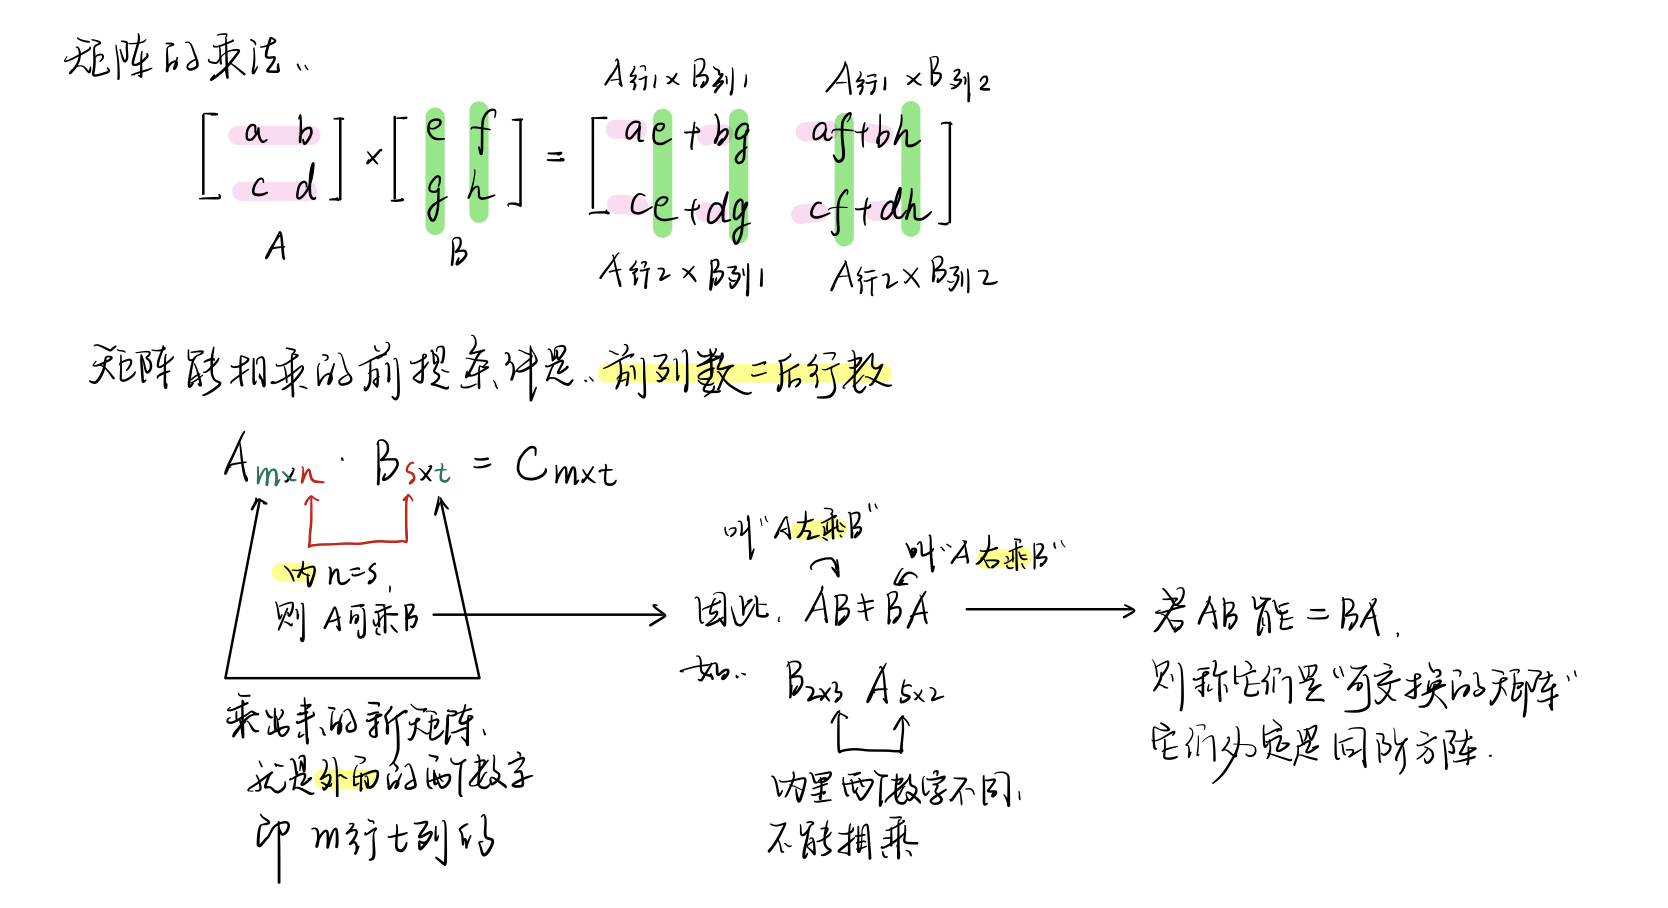
\includegraphics[width=1\textwidth]{img/0016.png} 

\begin{myEnvSample}
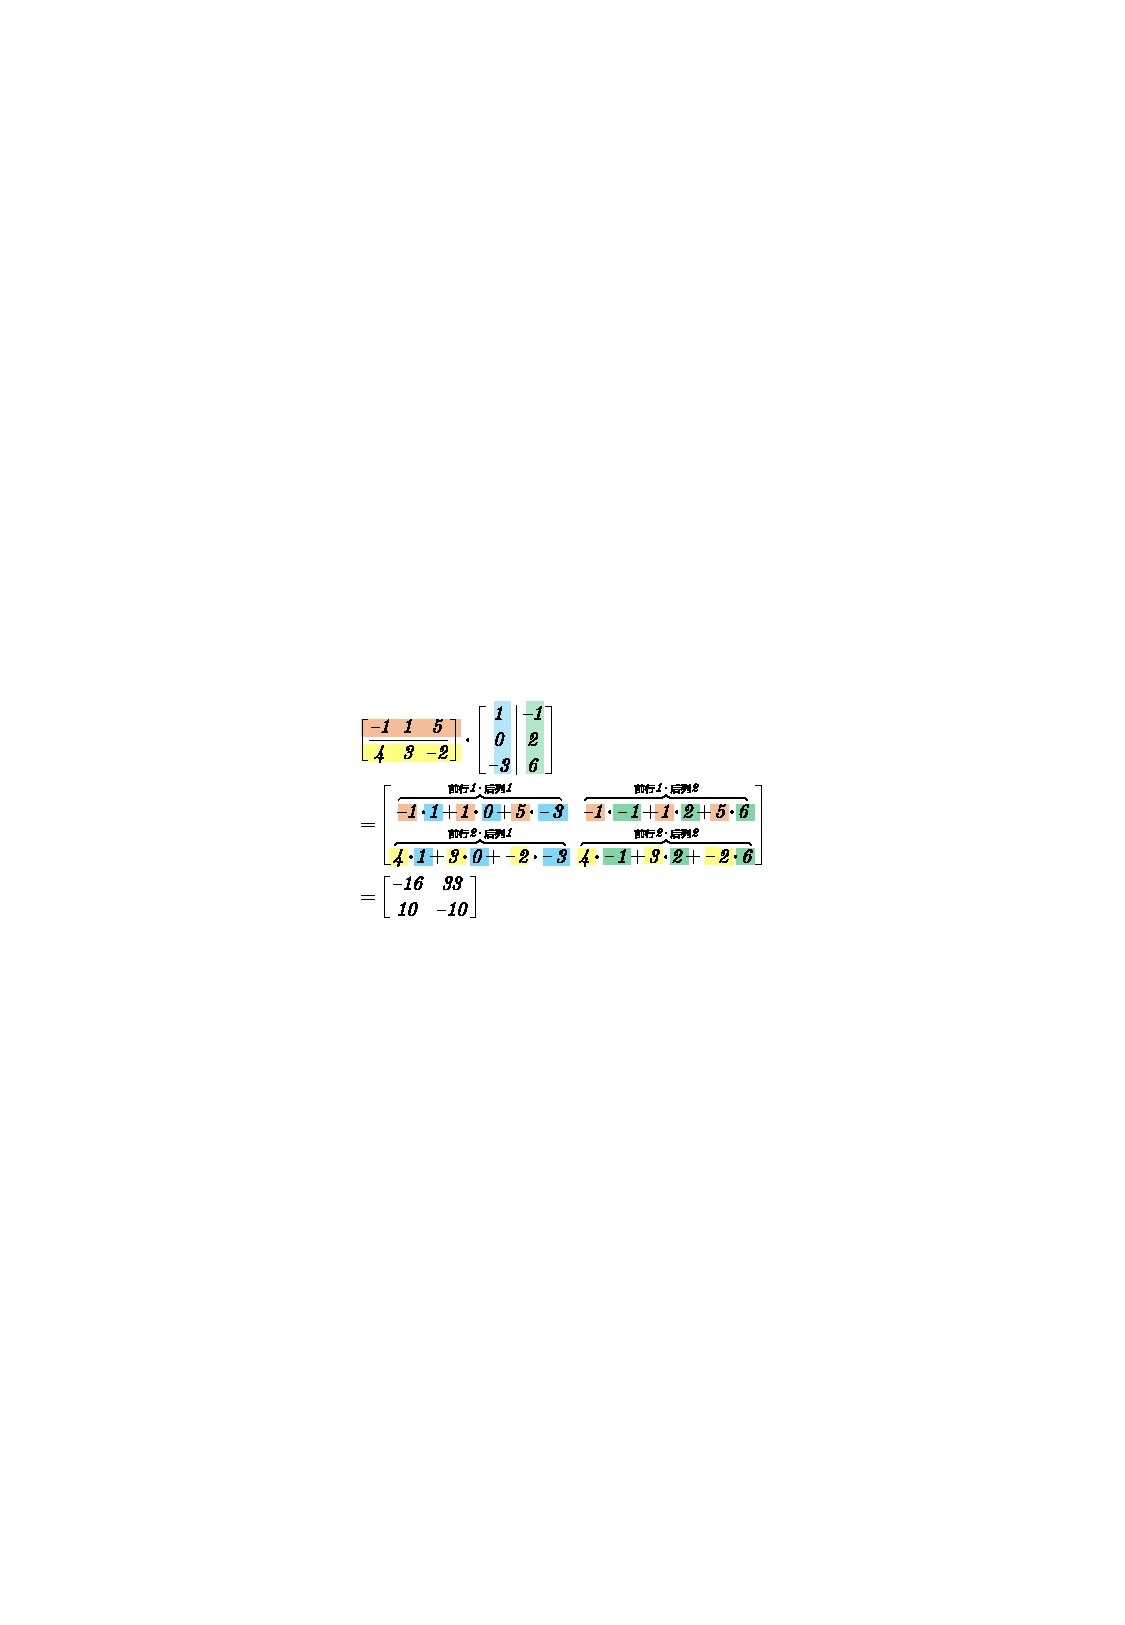
\includegraphics[width=0.6\textwidth]{img/0017.pdf}
\end{myEnvSample}



https://www.bilibili.com/video/BV1aW411Q7x1?p=9&vd_source=52c6cb2c1143f8e222795afbab2ab1b5

31.40

	--------------
	
	
	
	\part{线性方程组和矩阵}
	
	
	\part{矩阵的运算}
	
	\part{逆矩阵}
	
	\part{克拉默法则}
	
	\part{矩阵分块法}
	
\end{document}